\documentclass[pdf]{beamer}
\mode<presentation>{\usetheme{Singapore}}
\beamertemplatenavigationsymbolsempty
\title{Leader Election in Arbitrary, Asynchronous Networks}
\author{Michele Castrovilli, Mattia Cerrato, Pasha Ostadi}
\usepackage{default}
\usepackage{graphicx}
\graphicspath{{./img/}}
\usepackage{tcolorbox}
\usepackage{tikz}
\usetikzlibrary{arrows}

\begin{document}
\Large
\begin{frame}
    \maketitle
\end{frame}

\normalsize
\begin{frame}{Overview}
    \begin{itemize}
        \item Leader Election: a short review
        \item Floodmax in the asynchronous model
        \item Why use searching/tree building algorithms?
        \item Spanning trees
        \item Breadth-first search
        \item Bellman-Ford algorithm 
    \end{itemize}
\end{frame}

\section{Leader Election}
\begin{frame}{Leader Election}
    The leader is a node in the network that has to `take charge' of a computation
    
    \vspace{12pt}
    \pause
    All nodes have to agree on a single leader
    
    \vspace{12pt}
    \pause
    The criteria for choosing a leader is unimportant; usually the Process ID is used 
    
    \vspace{12pt}
    \pause
    We'll be tackling the leader election problem in an asynchronous arbitrary network 
\end{frame}

\section{Floodmax}
\begin{frame}{Synchronous Floodmax}
    \vspace{12pt}
    Each node knows the diameter \emph{diam} of the network, and has an unique identifier, UID. \\
    \pause
    For every round from 0 to \emph{diam}:  
    \pause
    \begin{enumerate}
        \item Send the maximum ID you found so far
        \pause
        \item Receive another ID, $ID_{2}$. If $ID_{2} >$ UID, \\
         UID $\leftarrow$ $ID_{2}$ 
    \end{enumerate}
    \pause
    After \emph{diam} rounds, every process will have the maximum UID of the network.
    If that UID corresponds to its own, the node will elect itself as the leader.
\end{frame}

\begin{frame}{Asynchronous Floodmax}{FloodMax}
    The FloodMax algorithm can be extended to the asynchronous network, by simulating
    the rounds.\\
    \pause
    \vspace{12pt}
    Each process sends a round r message to the neighbors, each process waits until 
    they received the round r message from every incoming neighbor. \\ 
    At that point, the node can prooced with the next round.\\
    \pause
    \vspace{12pt}
    Simulating \emph{diam} rounds, the algorithm can terminate correctly.
\end{frame}

\begin{frame}{Asynchronous Floodmax}{Simulation}
\begin{columns}
\begin{column}{.4\textwidth}
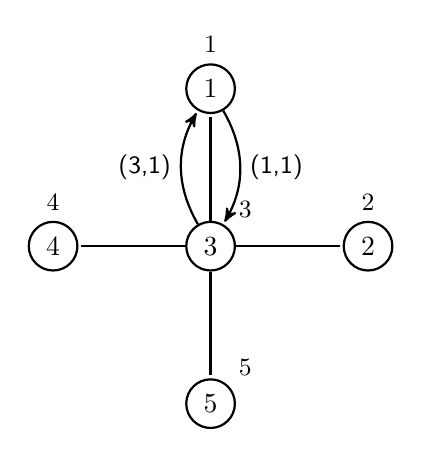
\begin{tikzpicture}[>=stealth',shorten >=1pt,auto,node distance=2cm,
                    thick,main node/.style={circle,draw,font=\normalsize}]
  \node[main node,label=above:{\small 1}] (1) {1};
  \node[main node,label=45:{\small 3}] (3) [below of=1] {3};
  \node[main node,label=above:{\small 2}] (2) [right of=3] {2};
  \node[main node,label=above:{\small 4}] (4) [left  of=3] {4};
  \node[main node,label=45:{\small 5}] (5) [below of=3] {5};
  \path[every node/.style={font=\sffamily\small}] 
    (1) edge [->,bend left] node [right] {(1,1)} (3)
    (3) edge [->,bend left] node [left] {(3,1)} (1)
    (3) edge node {} (1)
    (3) edge node {} (2)
    (3) edge node {} (4)
    (3) edge node {} (5)
    ;
\end{tikzpicture}
\end{column}
\vrule{}
\hspace*{10pt}
\begin{column}{.4\textwidth}
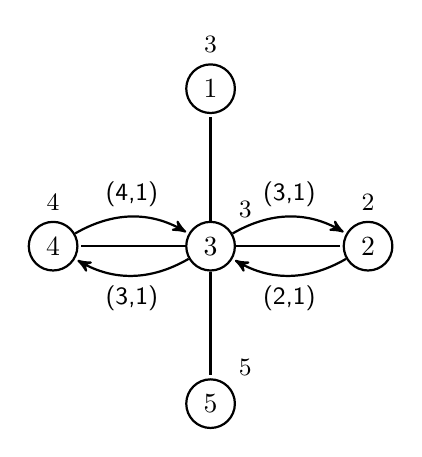
\begin{tikzpicture}[>=stealth',shorten >=1pt,auto,node distance=2cm,
                    thick,main node/.style={circle,draw,font=\normalsize}]
  \node[main node,label=above:{\small 3}] (1) {1};
  \node[main node,label=45:{\small 3}] (3) [below of=1] {3};
  \node[main node,label=above:{\small 2}] (2) [right of=3] {2};
  \node[main node,label=above:{\small 4}] (4) [left  of=3] {4};
  \node[main node,label=45:{\small 5}] (5) [below of=3] {5};
  \path[every node/.style={font=\sffamily\small}] 
    (2) edge [->,bend left] node [below] {(2,1)} (3)
    (3) edge [->,bend left] node [above] {(3,1)} (2)
    (4) edge [->,bend left] node [above] {(4,1)} (3)
    (3) edge [->,bend left] node [below] {(3,1)} (4)
    (3) edge node {} (1)
    (3) edge node {} (2)
    (3) edge node {} (4)
    (3) edge node {} (5)
    ;
\end{tikzpicture}
\end{column}
\end{columns}
\end{frame}

\begin{frame}{Asynchronous Floodmax}{Simulation}
\begin{columns}
\begin{column}{.4\textwidth}
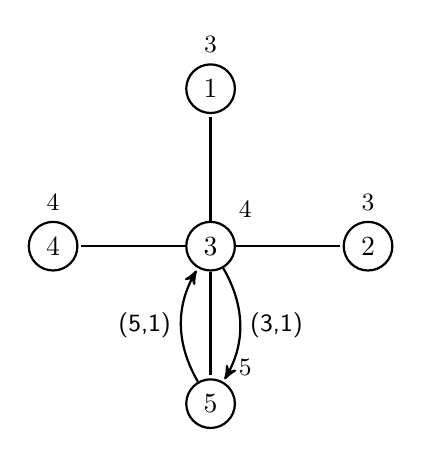
\begin{tikzpicture}[>=stealth',shorten >=1pt,auto,node distance=2cm,
                    thick,main node/.style={circle,draw,font=\normalsize}]
  \node[main node,label=above:{\small 3}] (1) {1};
  \node[main node,label=45:{\small 4}] (3) [below of=1] {3};
  \node[main node,label=above:{\small 3}] (2) [right of=3] {2};
  \node[main node,label=above:{\small 4}] (4) [left  of=3] {4};
  \node[main node,label=45:{\small 5}] (5) [below of=3] {5};
  \path[every node/.style={font=\sffamily\small}] 
    (5) edge [->,bend left] node [left] {(5,1)} (3)
    (3) edge [->,bend left] node [right] {(3,1)} (5)
    (3) edge node {} (1)
    (3) edge node {} (2)
    (3) edge node {} (4)
    (3) edge node {} (5)
    ;
\end{tikzpicture}
\end{column}
\vrule{}
\hspace*{10pt}
\begin{column}{.4\textwidth}
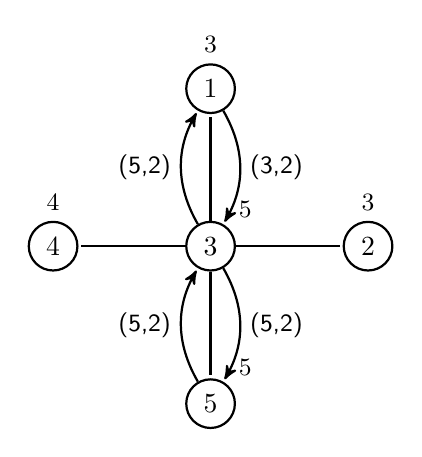
\begin{tikzpicture}[>=stealth',shorten >=1pt,auto,node distance=2cm,
                    thick,main node/.style={circle,draw,font=\normalsize}]
  \node[main node,label=above:{\small 3}] (1) {1};
  \node[main node,label=45:{\small 5}] (3) [below of=1] {3};
  \node[main node,label=above:{\small 3}] (2) [right of=3] {2};
  \node[main node,label=above:{\small 4}] (4) [left  of=3] {4};
  \node[main node,label=45:{\small 5}] (5) [below of=3] {5};
  \path[every node/.style={font=\sffamily\small}] 
    (5) edge [->,bend left] node [left] {(5,2)} (3)
    (3) edge [->,bend left] node [right] {(5,2)} (5)
    (1) edge [->,bend left] node [right] {(3,2)} (3)
    (3) edge [->,bend left] node [left] {(5,2)} (1)
    (3) edge node {} (1)
    (3) edge node {} (2)
    (3) edge node {} (4)
    (3) edge node {} (5)
    ;
\end{tikzpicture}
\end{column}
\end{columns}
\end{frame}

\begin{frame}{Asynchronous Floodmax}{Simulation}
\begin{columns}
\begin{column}{.4\textwidth}
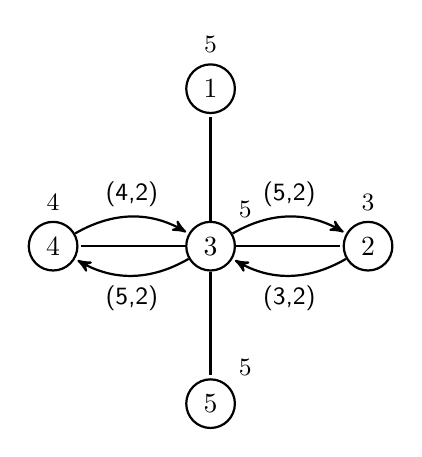
\begin{tikzpicture}[>=stealth',shorten >=1pt,auto,node distance=2cm,
                    thick,main node/.style={circle,draw,font=\normalsize}]
  \node[main node,label=above:{\small 5}] (1) {1};
  \node[main node,label=45:{\small 5}] (3) [below of=1] {3};
  \node[main node,label=above:{\small 3}] (2) [right of=3] {2};
  \node[main node,label=above:{\small 4}] (4) [left  of=3] {4};
  \node[main node,label=45:{\small 5}] (5) [below of=3] {5};
  \path[every node/.style={font=\sffamily\small}] 
    (4) edge [->,bend left] node [above] {(4,2)} (3)
    (3) edge [->,bend left] node [below] {(5,2)} (4)
    (2) edge [->,bend left] node [below] {(3,2)} (3)
    (3) edge [->,bend left] node [above] {(5,2)} (2)
    (3) edge node {} (1)
    (3) edge node {} (2)
    (3) edge node {} (4)
    (3) edge node {} (5)
    ;
\end{tikzpicture}
\end{column}
\vrule{}
\hspace*{10pt}
\begin{column}{.4\textwidth}
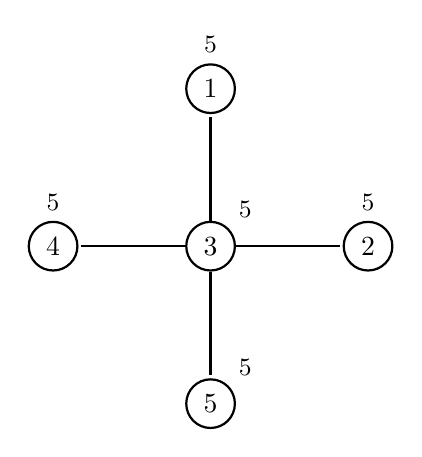
\begin{tikzpicture}[>=stealth',shorten >=1pt,auto,node distance=2cm,
                    thick,main node/.style={circle,draw,font=\normalsize}]
  \node[main node,label=above:{\small 5}] (1) {1};
  \node[main node,label=45:{\small 5}] (3) [below of=1] {3};
  \node[main node,label=above:{\small 5}] (2) [right of=3] {2};
  \node[main node,label=above:{\small 5}] (4) [left  of=3] {4};
  \node[main node,label=45:{\small 5}] (5) [below of=3] {5};
  \path[every node/.style={font=\sffamily\small}] 
    (3) edge node {} (1)
    (3) edge node {} (2)
    (3) edge node {} (4)
    (3) edge node {} (5)
    ;
\end{tikzpicture}
\end{column}
\end{columns}
\end{frame}

\begin{frame}{Asynchronous Floodmax}{OptFloodMax}
    An optimization for the synchronous case was shown, called \emph{OptFloodMax}.\\
    This optimization reduced greatly the number of messages sent.\\
    \pause
    \vspace{12pt}
    Each node sends to its neighbors an update of the maximum UID they know, only if
    it changed from the previous round.\\
    \pause
    \vspace{12pt}
    This cannot be ported to the asynchronous network, as the nodes cannot determine whether
    they received all the messages from the current round.\\
    \pause
    \vspace{12pt}
    Adding dummy messages to help processes determine the end of the round destroys the 
    optimization.
\end{frame}

\begin{frame}{Asynchronous Floodmax}{OptFloodMax Simulation}
\begin{center}
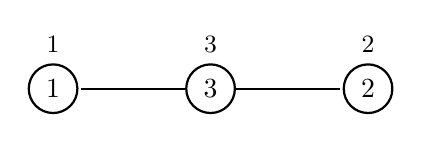
\begin{tikzpicture}[>=stealth',shorten >=1pt,auto,node distance=2cm,
                    thick,main node/.style={circle,draw,font=\normalsize}]
  \node[main node,label=above:{\small 1}] (1) {1};
  \node[main node,label=above:{\small 3}] (3) [right of=1] {3};
  \node[main node,label=above:{\small 2}] (2) [right of=3] {2};
  \path[every node/.style={font=\sffamily\small}] 
    (3) edge node {} (1)
    (3) edge node {} (2)
    ;
\end{tikzpicture}
\end{center}
\end{frame}

\begin{frame}{Asynchronous Floodmax}{OptFloodMax Simulation}
\begin{center}
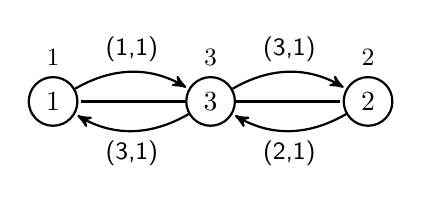
\begin{tikzpicture}[>=stealth',shorten >=1pt,auto,node distance=2cm,
                    thick,main node/.style={circle,draw,font=\normalsize}]
  \node[main node,label=above:{\small 1}] (1) {1};
  \node[main node,label=above:{\small 3}] (3) [right of=1] {3};
  \node[main node,label=above:{\small 2}] (2) [right of=3] {2};
  \path[every node/.style={font=\sffamily\small}] 
    (3) edge node {} (1)
    (3) edge node {} (2)
    (1) edge [->,bend left] node [above] {(1,1)} (3)
    (3) edge [->,bend left] node [below] {(3,1)} (1)
    (2) edge [->,bend left] node [below] {(2,1)} (3)
    (3) edge [->,bend left] node [above] {(3,1)} (2)
    ;
\end{tikzpicture}
\end{center}
\end{frame}

\begin{frame}{Asynchronous Floodmax}{OptFloodMax Simulation}
\begin{center}
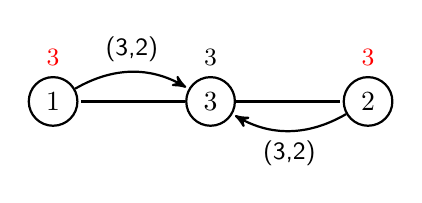
\begin{tikzpicture}[>=stealth',shorten >=1pt,auto,node distance=2cm,
                    thick,main node/.style={circle,draw,font=\normalsize}]
  \node[main node,label={[red]above:{\small 3}}] (1) {1};
  \node[main node,label={above:{\small 3}}] (3) [right of=1] {3};
  \node[main node,label={[red]above:{\small 3}}] (2) [right of=3] {2};
  \path[every node/.style={font=\sffamily\small}] 
    (3) edge node {} (1)
    (3) edge node {} (2)
    (1) edge [->,bend left] node [above] {(3,2)} (3)
    (2) edge [->,bend left] node [below] {(3,2)} (3)
    ;
\end{tikzpicture}
\end{center}
Since the nodes 1 and 2 do not receive the message for the round from 3, they never finish round 2.
\end{frame}

\begin{frame}{Asynchronous Floodmax}{OptFloodMax}
    The algorithm can be run purely asynchronously, without rounds.\\
    The processes will propagate UIDs only when they receive a greater one.\\
    \pause
    \vspace{12pt}
    This strategy will eventually propagate the maximum.\\
    \pause
    \vspace{12pt}
    The processes do not know when to terminate.
\end{frame}

\begin{frame}{What can we do?}
    There are different solutions to this problem.\\
    \vspace{12pt}
    We'll be looking at the \emph{Asynchronous broadcast and convergecast, based on breadth-first search}.\\
    \vspace{12pt}
    To solve the leader election problem, we'll start from a spanning tree.
\end{frame}

\section{Spanning Tree}
\begin{frame}{Asynchronous Spanning Tree}{Why?}
    A spanning tree allows for a process to implement broadcast and convergecast on
    an arbitrary network that allows for only point to point communication.\\
    \vspace{12pt}
    By having an unrooted spanning tree, we can also implement a leader election 
    easily.
\end{frame}

\begin{frame}{Asynchronous Spanning Tree}{STtoLeader}
    The algorithm uses a convergecast of \emph{elect} messages starting from the leaves.\\
    Each leaf node sends an \emph{elect} message to the unique neighbor.\\
    If a node receives \emph{elect} messages from all its neighbors except one, it 
    then sends an \emph{elect} message to that neighbor.\\
    \vspace{12pt}
    In the end, we have two cases:
    \begin{itemize}
        \item{If a process receives \emph{elect} messages on every channel before
              sending an \emph{elect} message themselves, it elects themselves as a leader.}
        \item{If two \emph{elect} messages are sent on some edge in both directions, then
          one of the two processes at the endpoints will elect itself as a leader, based 
          on some condition (e.g., larger UID).}
    \end{itemize}
\end{frame}

\begin{frame}{Asynchronous Spanning Tree}{STtoLeader Results}
    Message complexity: \emph{n}.\\
    Time complexity: $\mathcal{O}(n*(l+d))$.\\
    \vspace{12pt}
    $n$ is the number of nodes in the graph.\\
    $l$ is the upper bound for each task in the process to be completed.
    $d$ is the upper bound for a message to be passed through the channel.
\end{frame}

\begin{frame}{Asynchronous Spanning Tree}{Base Algorithm}
    The \emph{AsynchSpanningTree} algorithm works on the premises:
    \begin{itemize}
        \item{The graph is undirected and connected.}
        \pause
        \item{There is a marked node $i_0$.}
    \end{itemize}
    \vspace{12pt}
    \pause
    Search messages start from $i_0$ and propagate throughout the network.\\
    \pause
    \vspace{12pt}
    A node receiving a search message from $i$, denotes $i$ as the parent, and
    propagates the search message to its neighbors.
\end{frame}

\begin{frame}{Asynchronous Spanning Tree}{Simulation}
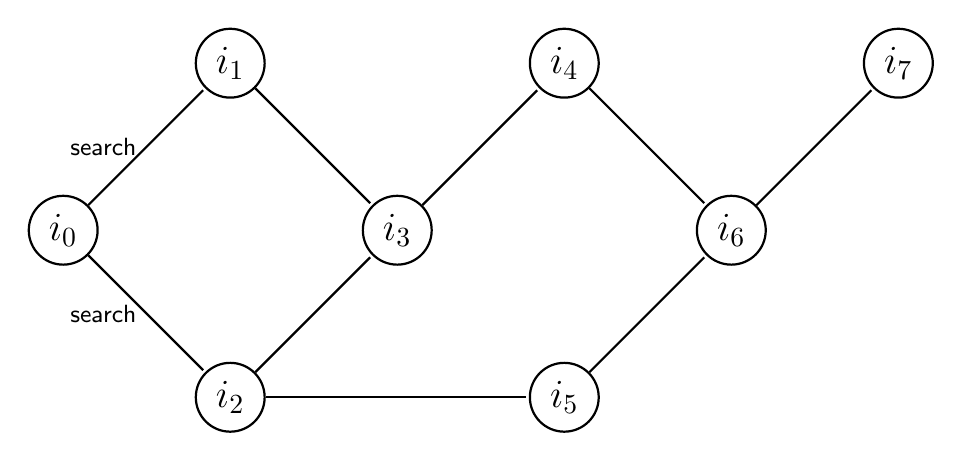
\begin{tikzpicture}[>=stealth',shorten >=1pt,auto,node distance=3cm,
                    thick,main node/.style={circle,draw,font=\sffamily\Large\bfseries}]
  \node[main node] (1) {$i_0$};
  \node[main node] (2) [above right of=1] {$i_1$};
  \node[main node] (3) [below right of=1] {$i_2$};
  \node[main node] (4) [below right of=2] {$i_3$};
  \node[main node] (5) [above right of=4] {$i_4$};
  \node[main node] (6) [below right of=4] {$i_5$};
  \node[main node] (7) [above right of=6] {$i_6$};
  \node[main node] (8) [above right of=7] {$i_7$};
  \path[every node/.style={font=\sffamily\small}]
    (1) edge node [left] {search} (2)
        edge node [left] {search} (3)
    (2) edge node [left] {} (4)
    (3) edge node [left] {} (4)
    (3) edge node [left] {} (6)
    (4) edge node [left] {} (5)
    (5) edge node [left] {} (7)
    (6) edge node [left] {} (7)
    (7) edge node [left] {} (8);
\end{tikzpicture}
\end{frame}

\begin{frame}{Asynchronous Spanning Tree}{Simulation}
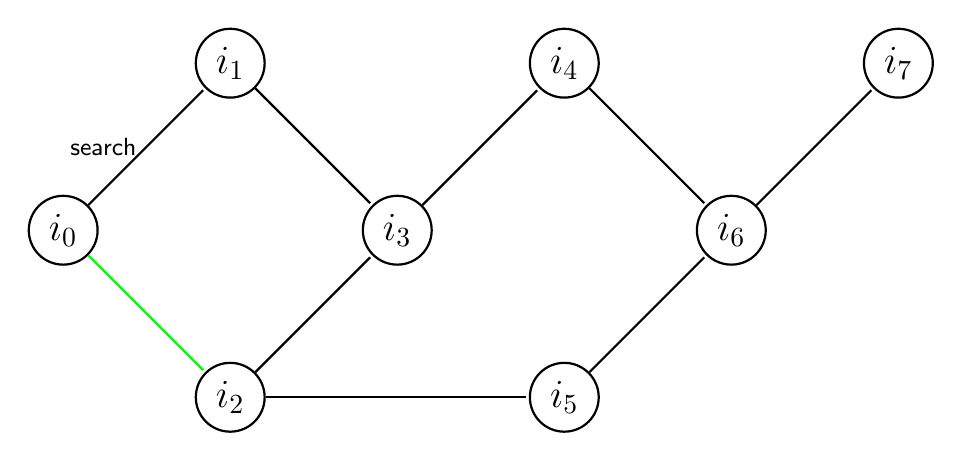
\begin{tikzpicture}[>=stealth',shorten >=1pt,auto,node distance=3cm,
                    thick,main node/.style={circle,draw,font=\sffamily\Large\bfseries}]
  \node[main node] (1) {$i_0$};
  \node[main node] (2) [above right of=1] {$i_1$};
  \node[main node] (3) [below right of=1] {$i_2$};
  \node[main node] (4) [below right of=2] {$i_3$};
  \node[main node] (5) [above right of=4] {$i_4$};
  \node[main node] (6) [below right of=4] {$i_5$};
  \node[main node] (7) [above right of=6] {$i_6$};
  \node[main node] (8) [above right of=7] {$i_7$};
  \path[every node/.style={font=\sffamily\small}]
    (1) edge node [left] {search} (2)
        edge [draw=green] node [left] {} (3)
    (2) edge node [left] {} (4)
    (3) edge node [left] {} (4)
    (3) edge node [left] {} (6)
    (4) edge node [left] {} (5)
    (5) edge node [left] {} (7)
    (6) edge node [left] {} (7)
    (7) edge node [left] {} (8);
\end{tikzpicture}
\end{frame}

\begin{frame}{Asynchronous Spanning Tree}{Simulation}
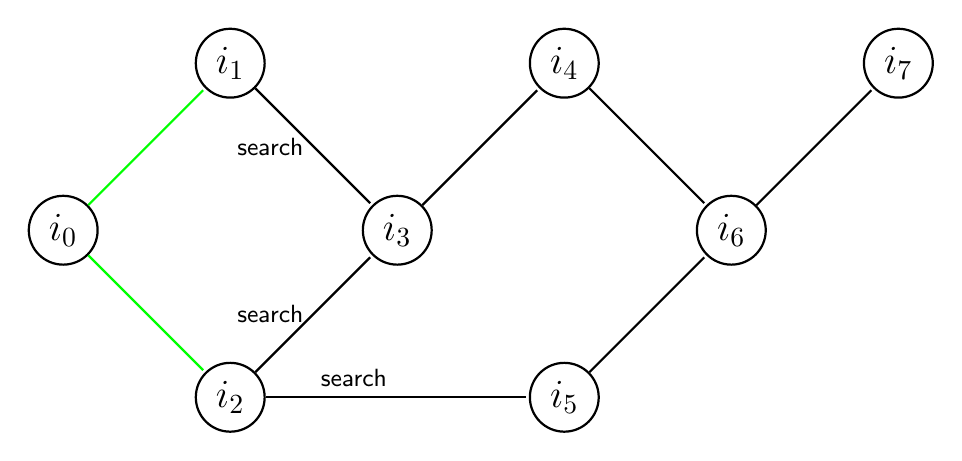
\begin{tikzpicture}[>=stealth',shorten >=1pt,auto,node distance=3cm,
                    thick,main node/.style={circle,draw,font=\sffamily\Large\bfseries}]
  \node[main node] (1) {$i_0$};
  \node[main node] (2) [above right of=1] {$i_1$};
  \node[main node] (3) [below right of=1] {$i_2$};
  \node[main node] (4) [below right of=2] {$i_3$};
  \node[main node] (5) [above right of=4] {$i_4$};
  \node[main node] (6) [below right of=4] {$i_5$};
  \node[main node] (7) [above right of=6] {$i_6$};
  \node[main node] (8) [above right of=7] {$i_7$};
  \path[every node/.style={font=\sffamily\small}]
    (1) edge [draw=green] node [left] {} (2)
        edge [draw=green] node [left] {} (3)
    (2) edge node [left] {search} (4)
    (3) edge node [left] {search} (4)
    (3) edge node [above left] {search} (6)
    (4) edge node [left] {} (5)
    (5) edge node [left] {} (7)
    (6) edge node [left] {} (7)
    (7) edge node [left] {} (8);
\end{tikzpicture}
\end{frame}

\begin{frame}{Asynchronous Spanning Tree}{Simulation}
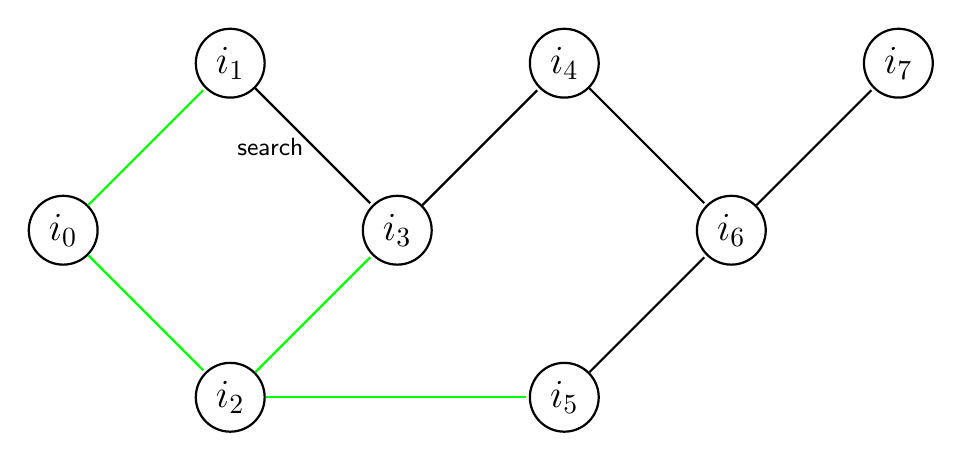
\begin{tikzpicture}[>=stealth',shorten >=1pt,auto,node distance=3cm,
                    thick,main node/.style={circle,draw,font=\sffamily\Large\bfseries}]
  \node[main node] (1) {$i_0$};
  \node[main node] (2) [above right of=1] {$i_1$};
  \node[main node] (3) [below right of=1] {$i_2$};
  \node[main node] (4) [below right of=2] {$i_3$};
  \node[main node] (5) [above right of=4] {$i_4$};
  \node[main node] (6) [below right of=4] {$i_5$};
  \node[main node] (7) [above right of=6] {$i_6$};
  \node[main node] (8) [above right of=7] {$i_7$};
  \path[every node/.style={font=\sffamily\small}]
    (1) edge [draw=green] node [left] {} (2)
        edge [draw=green] node [left] {} (3)
    (2) edge node [left] {search} (4)
    (3) edge [draw=green] node [left] {} (4)
    (3) edge [draw=green] node [below left] {} (6)
    (4) edge node [left] {} (5)
    (5) edge node [left] {} (7)
    (6) edge node [left] {} (7)
    (7) edge node [left] {} (8);
\end{tikzpicture}
\end{frame}

\begin{frame}{Asynchronous Spanning Tree}{Simulation}
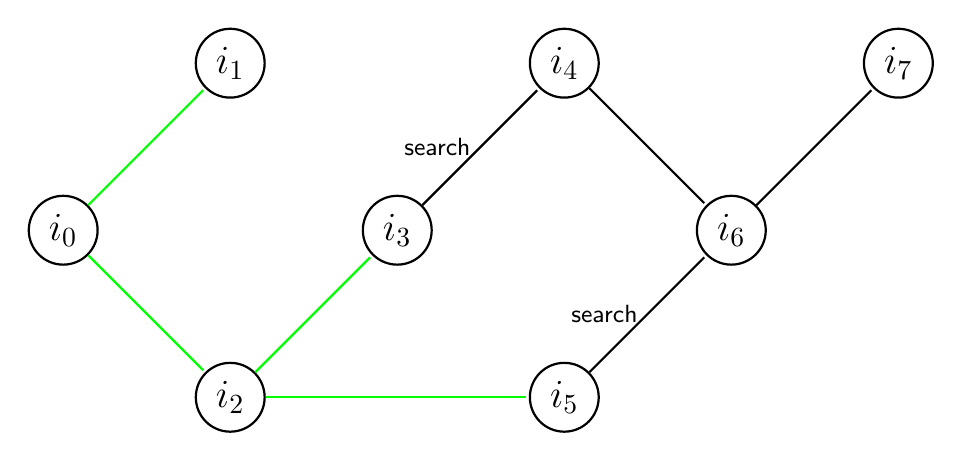
\begin{tikzpicture}[>=stealth',shorten >=1pt,auto,node distance=3cm,
                    thick,main node/.style={circle,draw,font=\sffamily\Large\bfseries}]
  \node[main node] (1) {$i_0$};
  \node[main node] (2) [above right of=1] {$i_1$};
  \node[main node] (3) [below right of=1] {$i_2$};
  \node[main node] (4) [below right of=2] {$i_3$};
  \node[main node] (5) [above right of=4] {$i_4$};
  \node[main node] (6) [below right of=4] {$i_5$};
  \node[main node] (7) [above right of=6] {$i_6$};
  \node[main node] (8) [above right of=7] {$i_7$};
  \path[every node/.style={font=\sffamily\small}]
    (1) edge [draw=green] node [left] {} (2)
        edge [draw=green] node [left] {} (3)
    (3) edge [draw=green] node [left] {} (4)
    (3) edge [draw=green] node [below left] {} (6)
    (4) edge node [left] {search} (5)
    (5) edge node [left] {} (7)
    (6) edge node [left] {search} (7)
    (7) edge node [left] {} (8);
\end{tikzpicture}
\end{frame}

\begin{frame}{Asynchronous Spanning Tree}{Simulation}
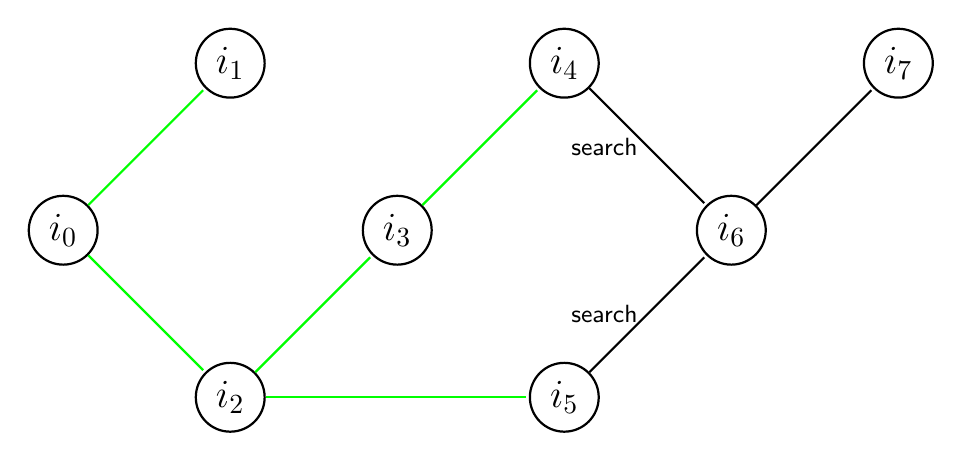
\begin{tikzpicture}[>=stealth',shorten >=1pt,auto,node distance=3cm,
                    thick,main node/.style={circle,draw,font=\sffamily\Large\bfseries}]
  \node[main node] (1) {$i_0$};
  \node[main node] (2) [above right of=1] {$i_1$};
  \node[main node] (3) [below right of=1] {$i_2$};
  \node[main node] (4) [below right of=2] {$i_3$};
  \node[main node] (5) [above right of=4] {$i_4$};
  \node[main node] (6) [below right of=4] {$i_5$};
  \node[main node] (7) [above right of=6] {$i_6$};
  \node[main node] (8) [above right of=7] {$i_7$};
  \path[every node/.style={font=\sffamily\small}]
    (1) edge [draw=green] node [left] {} (2)
        edge [draw=green] node [left] {} (3)
    (3) edge [draw=green] node [left] {} (4)
    (3) edge [draw=green] node [below left] {} (6)
    (4) edge [draw=green] node [left] {} (5)
    (5) edge node [left] {search} (7)
    (6) edge node [left] {search} (7)
    (7) edge node [left] {} (8);
\end{tikzpicture}
\end{frame}

\begin{frame}{Asynchronous Spanning Tree}{Simulation}
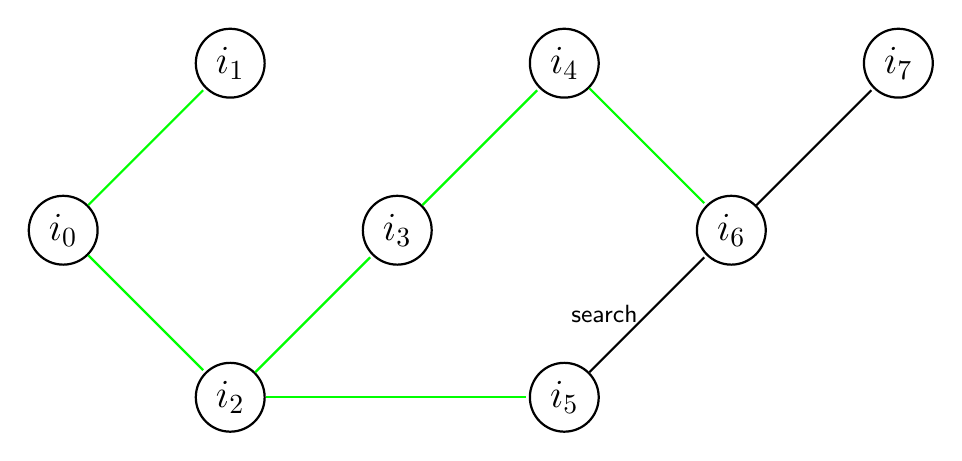
\begin{tikzpicture}[>=stealth',shorten >=1pt,auto,node distance=3cm,
                    thick,main node/.style={circle,draw,font=\sffamily\Large\bfseries}]
  \node[main node] (1) {$i_0$};
  \node[main node] (2) [above right of=1] {$i_1$};
  \node[main node] (3) [below right of=1] {$i_2$};
  \node[main node] (4) [below right of=2] {$i_3$};
  \node[main node] (5) [above right of=4] {$i_4$};
  \node[main node] (6) [below right of=4] {$i_5$};
  \node[main node] (7) [above right of=6] {$i_6$};
  \node[main node] (8) [above right of=7] {$i_7$};
  \path[every node/.style={font=\sffamily\small}]
    (1) edge [draw=green] node [left] {} (2)
        edge [draw=green] node [left] {} (3)
    (3) edge [draw=green] node [left] {} (4)
    (3) edge [draw=green] node [below left] {} (6)
    (4) edge [draw=green] node [left] {} (5)
    (5) edge [draw=green] node [left] {} (7)
    (6) edge node [left] {search} (7)
    (7) edge node [left] {} (8);
\end{tikzpicture}
\end{frame}

\begin{frame}{Asynchronous Spanning Tree}{Simulation}
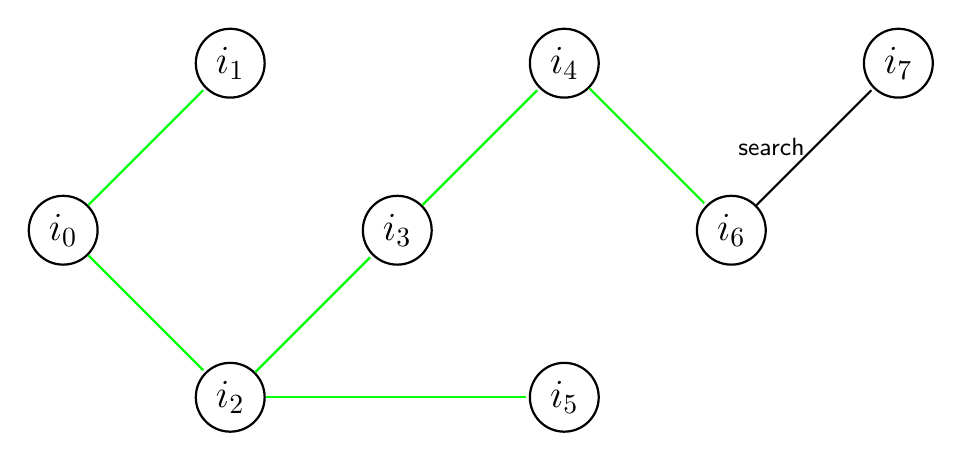
\begin{tikzpicture}[>=stealth',shorten >=1pt,auto,node distance=3cm,
                    thick,main node/.style={circle,draw,font=\sffamily\Large\bfseries}]
  \node[main node] (1) {$i_0$};
  \node[main node] (2) [above right of=1] {$i_1$};
  \node[main node] (3) [below right of=1] {$i_2$};
  \node[main node] (4) [below right of=2] {$i_3$};
  \node[main node] (5) [above right of=4] {$i_4$};
  \node[main node] (6) [below right of=4] {$i_5$};
  \node[main node] (7) [above right of=6] {$i_6$};
  \node[main node] (8) [above right of=7] {$i_7$};
  \path[every node/.style={font=\sffamily\small}]
    (1) edge [draw=green] node [left] {} (2)
        edge [draw=green] node [left] {} (3)
    (3) edge [draw=green] node [left] {} (4)
    (3) edge [draw=green] node [below left] {} (6)
    (4) edge [draw=green] node [left] {} (5)
    (5) edge [draw=green] node [left] {} (7)
    (7) edge node [left] {search} (8);
\end{tikzpicture}
\end{frame}

\begin{frame}{Asynchronous Spanning Tree}{Simulation}
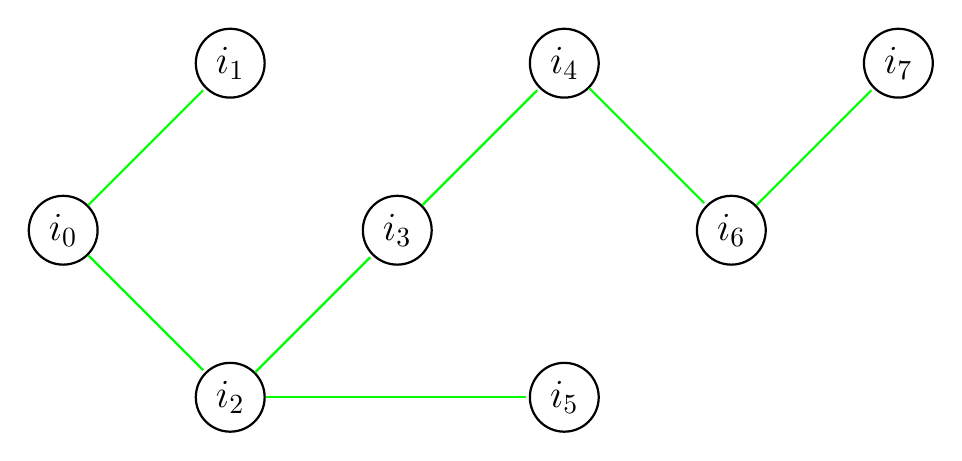
\begin{tikzpicture}[>=stealth',shorten >=1pt,auto,node distance=3cm,
                    thick,main node/.style={circle,draw,font=\sffamily\Large\bfseries}]
  \node[main node] (1) {$i_0$};
  \node[main node] (2) [above right of=1] {$i_1$};
  \node[main node] (3) [below right of=1] {$i_2$};
  \node[main node] (4) [below right of=2] {$i_3$};
  \node[main node] (5) [above right of=4] {$i_4$};
  \node[main node] (6) [below right of=4] {$i_5$};
  \node[main node] (7) [above right of=6] {$i_6$};
  \node[main node] (8) [above right of=7] {$i_7$};
  \path[every node/.style={font=\sffamily\small}]
    (1) edge [draw=green] node [left] {} (2)
        edge [draw=green] node [left] {} (3)
    (3) edge [draw=green] node [left] {} (4)
    (3) edge [draw=green] node [below left] {} (6)
    (4) edge [draw=green] node [left] {} (5)
    (5) edge [draw=green] node [left] {} (7)
    (7) edge [draw=green] node [left] {} (8);
\end{tikzpicture}
\end{frame}

\begin{frame}{Asynchronous Spanning Tree}{Algorithm}
	$AsynchSpanningTree_i$
    \begin{block}{Signature}
        \begin{columns}
            \column{.5\textwidth}
            Input:\\
            \hspace*{2pt} 
              {$receive("search")_{j,i}, j \in nbrs$}
            \column{.5\textwidth}
            Output:
            \hspace*{2pt}
            \parbox{\textwidth}{$send("search")_{i,j}, j \in nbrs$\\
               $parent(j)_i, j \in nbrs$}
        \end{columns}
    \end{block}
    \begin{block}{States}
        $parent \in nbrs \cup \{null\}$, initially $null$\\
        $reported$, a Boolean, initially $false$\\
        for every $j \in nbrs$:\\
        \hspace*{2pt}
        \parbox{\textwidth}{$send(j) \in \{search,null\}$,
        initially $search$ if $i=i_0$, else $null$}
    \end{block}
\end{frame}

\begin{frame}{Asynchronous Spanning Tree}{Algorithm}
    \begin{block}{Transitions}
        \begin{columns}[t]
            \column{.5\textwidth}
            $send("search")_{i,j}$ \\
            \hspace*{2pt} {Precondition:} \\
            \hspace*{5pt} {$send(j) = search$} \\
            \hspace*{2pt} {Effect:} \\
            \hspace*{5pt} {$send(j) := search$} \\
            \vspace{12pt}
            $receive("search")_{j,i}$ \\
            \hspace*{2pt} {Effect:} \\
            \hspace*{5pt} {if $i \neq i_0$ and $parent = null$ then}\\
            \hspace*{7pt} {$parent := j$} \\
            \hspace*{7pt} {for all $k \in nbrs - \{j\}$ do} \\
            \hspace*{9pt} {$send(k) := search$} 
            \column{.5\textwidth}
            $parent(j)_{i}$ \\
            \hspace*{2pt} {Precondition:} \\
            \hspace*{5pt} {$parent = j$} \\
            \hspace*{5pt} {$reported = false$} \\
            \hspace*{2pt} {Effect:} \\
            \hspace*{5pt} {$reported := true$} 
        \end{columns}
    \end{block}
    \vskip-3cm
    \begin{columns}
     \column{.5\textwidth}
    \column{.5\textwidth}
    \begin{block}{Tasks}
    $\{parent(j)_i : j \in nbrs\}$\\
    for every $j \in nbrs$: \\
        \hspace*{2pt}
        \parbox{\textwidth}{$\{send("search")_{i,j}\}$}
    \end{block}
    \end{columns}
\end{frame}

\begin{frame}[plain]{Asynchronous Spanning Tree}{Proof}
    \begin{block}{Assertion 1}
    In any reachable state, the edges defined by all the parent variables form a spanning tree
    of a subgraph of $G$, containing $i_0$; moreover, if there is a message in any channel $C_{i,j}$,
    then $i$ is in this spanning tree.
    \end{block}	
    \pause
    \begin{block}{Proof - Base case (will be reduced, along with blackboard explaining)}
    The first part is trivially proven,
    as there are no parent variables, and $G$ contains $i_0$ by definition.\\
    Second part, we have search messages starting only from $i_0$, by the algorithm definition.\\
    \end{block}
\end{frame}

\begin{frame}[plain]{Asynchronous Spanning Tree}{Proof}
    \begin{block}{Assertion 1}
    In any reachable state, the edges defined by all the parent variables form a spanning tree
    of a subgraph of $G$, containing $i_0$; moreover, if there is a message in any channel $C_{i,j}$,
    then $i$ is in this spanning tree.
    \end{block}	
    \begin{block}{Proof - Inductive step (will be reduced, along with blackboard explaining)}
    We look at each transition, and how it does not change the invariant.
    \begin{description}
    \item[$send$]{Since the send transition sends a message from the node i to the neighbors, we need
        to prove that i is in the spanning tree. By the algorithm, the send transition has the precondition of the $send(j)$ variable, which is set only as the node enters the spanning tree.}
    \end{description}
    \end{block}
\end{frame}

\begin{frame}[plain]{Asynchronous Spanning Tree}{Proof}
    \begin{block}{Assertion 1}
    In any reachable state, the edges defined by all the parent variables form a spanning tree
    of a subgraph of $G$, containing $i_0$; moreover, if there is a message in any channel $C_{i,j}$,
    then $i$ is in this spanning tree.
    \end{block}	
    \begin{block}{Proof - Inductive step (will be reduced, along with blackboard explaining)}
    \begin{description}
    \item[$receive$]{\small The receive of a search message to a node not in the spanning tree, allows for the node to enter the spanning tree by setting the parent variable to the neighbor that sent the message. It then sets the variables in order to send the search message to the remaining neighbors.\\
        If the node already has the parent variable set, it discards the message. 
    Since this only adds a node, $i_0$ is still contained in the spanning tree.}
    \end{description}
    \end{block}
\end{frame}

\begin{frame}[plain]{Asynchronous Spanning Tree}{Proof}
    \begin{block}{Assertion 1}
    In any reachable state, the edges defined by all the parent variables form a spanning tree
    of a subgraph of $G$, containing $i_0$; moreover, if there is a message in any channel $C_{i,j}$,
    then $i$ is in this spanning tree.
    \end{block}	
    \begin{block}{Proof - Inductive step (will be reduced, along with blackboard explaining)}
    \begin{description}
    \item[$parent$]{The parent action will activate once, as the parent variable is set, reporting the node's presence in the spanning tree.}
    \end{description}
    \end{block}
\end{frame}

\begin{frame}[plain]{Asynchronous Spanning Tree}{Proof}
    \begin{block}{Assertion 2 - Liveness}
        In any reachable state, if $i=i_0$ or $parent_i \neq null$, and if $j \in nbrs_i - \{i_0\}$,
        then either $parent_j \neq null$ or $C_{i,j}$ contains a $search$ message or $send(j)_i$ contains a $search$ message.
    \end{block}	
    \begin{block}{Proof - Base step (will be reduced, along with blackboard explaining)}
    As the initial state, we have that every $parent_i = null$, so we need to only check $i_0$.
    As the initial state, $i_0$ has that for all its neighbors $send(j)_i$ contains a search message,
    therefore proving the invariant.
    \end{block}
\end{frame}
\begin{frame}[plain]{Asynchronous Spanning Tree}{Proof}
    \begin{block}{Assertion 2 - Liveness}
        In any reachable state, if $i=i_0$ or $parent_i \neq null$, and if $j \in nbrs_i - \{i_0\}$,
        then either $parent_j \neq null$ or $C_{i,j}$ contains a $search$ message or $send(j)_i$ contains a $search$ message.
    \end{block}	
    \begin{block}{Proof - Inductive step (will be reduced, along with blackboard explaining)}
    We look at each transition, and show how it doesn't invalidate the invariant.
    \begin{description}
    \item[$send$]{As the effect will remove the $search$ message from the $send(j)$ variable, the channel $C_{i,j}$ will now contain a $search$ message instead.}
    \end{description}
    \end{block}
\end{frame}
\begin{frame}[plain]{Asynchronous Spanning Tree}{Proof}
    \begin{block}{Assertion 2 - Liveness}
        In any reachable state, if $i=i_0$ or $parent_i \neq null$, and if $j \in nbrs_i - \{i_0\}$,
        then either $parent_j \neq null$ or $C_{i,j}$ contains a $search$ message or $send(j)_i$ contains a $search$ message.
    \end{block}	
    \begin{block}{Proof - Inductive step (will be reduced, along with blackboard explaining)}
    \begin{description}
    \item[$receive$]{As $parent_i$ becomes different than $null$, for each $j \in nbrs - {parent_i}$,
    it will set $send(j) = search$. For $parent_i$ instead, we can already prove from the first assertion that since a message came from $parent_i$ it must be in the spanning tree, and so its $parent$ variable different than $null$.}
    \item[$parent$]{It doesn't affect any of the variables in the assertion.}
    \end{description}
    \end{block}
\end{frame}
\begin{frame}[plain]{Asynchronous Spanning Tree}{Proof}
    \begin{block}{Assertion 1}
    In any reachable state, the edges defined by all the parent variables form a spanning tree
    of a subgraph of $G$, containing $i_0$; moreover, if there is a message in any channel $C_{i,j}$,
    then $i$ is in this spanning tree.
    \end{block}	
    \begin{block}{Assertion 2 - Liveness}
        In any reachable state, if $i=i_0$ or $parent_i \neq null$, and if $j \in nbrs_i - \{i_0\}$,
        then either $parent_j \neq null$ or $C_{i,j}$ contains a $search$ message or $send(j)_i$ contains a $search$ message.
    \end{block}	
    \begin{block}{Conclusions}
        From these two assertions we can then argue that the algorithm constructs a spanning tree.\\
        Furthermore, for any $i \neq i_0$ we have $parent_i \neq null$ within time $distance(i_0,i)\cdot(l+d)$, which implies the liveness.
    \end{block}
\end{frame}
\begin{frame}{Asynchronous Spanning Tree}{Results}
    Number of messages: $\mathcal{O}(|E|)$.\\
    Time upper bound for all processes except $i_0$: $diam(l+d)+l$.\\
    \vspace{6pt}
    $|E|$ is the number of edges in the graph.\\
    $n$ is the number of nodes in the graph.\\
    $l$ is the upper bound for each task in the process to be completed.\\
    $d$ is the upper bound for a message to be passed through the channel.\\
    \pause
    \vspace{6pt}
    The paths might be longer than the diameter, nonetheless the time is still bounded in 
    terms of diameter, because the time of the shortest path might be greater than the 
    fastest one.
\end{frame}

\begin{frame}{Asynchronous Spanning Tree}{Broadcast and Child Pointers}
    \begin{block}{Broadcast}
        It's easy to modify the algorithm, as we use a method of \emph{piggybacking} on the
        $search$ message. It also shares the complexities as the spanning tree algorithm.
    \end{block}
    \begin{block}{Child Pointers}
        Since the graph is assumed to be undirected, it's easy for the children to reply
        directly to the parent, in order for the parent to acknowledge them, or not.\\
        This can also implement \emph{broadcasting}.\\
        The complexity of the approach is $\mathcal{O}(n)$ per broadcast, and time complexity
        $\mathcal{O}(h(l+d))$ where $h$ is the height of the spanning tree, which is might be bounded
        as $\mathcal{O}(n(l+d))$ if a \emph{AsynchSpanningTree} was used, as the height might be bigger than the diameter. \\
    \end{block}
\end{frame}

\begin{frame}{Asynchronous Spanning Tree}{Broadcast and Child Pointers}
    \begin{block}{Child Pointers}
        The spanning tree with child pointers can also be used for \emph{convergecast}, with the same complexities as the broadcast.\\
        The two can be combined in a broadcast, followed by a convergecast to acknowledge the receival.
    \end{block}
    \begin{block}{Leader Election}
        By allowing every node to initiate a broadcast-convergecast, and having UIDs, we can also solve the leader election problem, with every node discovering the maximum UID in the network, and then electing itself as a leader if the maximum UID equals to its own.\\
        The message complexity of this approach is $\mathcal{O}(n|E|)$.
    \end{block}
\end{frame}

\section{Breadth-First Search}
\begin{frame}{Breadth-First Search}{Problem}
	Another way to build a Spanning Tree is via Breadth-First Search. \\
    \vspace{12pt}
    \pause
    As in the synchronous setting, we can also find the shortest paths, so that each node is reached in the least amount of edges. \emph{(We are not taking weights into account just yet.)} \\
    \vspace{12pt}
    \pause
    We require a starting node $i_0$.
\end{frame}

\begin{frame}{Breadth-First Search}{Problem}
    To find the shortest paths in a distributed manner, the nodes have to change their parent designations if they are reached along a shorter path. If this happens, they also have to propagate this information to their neighbors, so that they may change their parents. \\
    \vspace{12pt}
    \pause
    However, there is no way to guarantee termination: each node has to wait indefinitely to see if it can obtain a closer parent. \\
    \vspace{12pt}
    \pause
    Even if a Spanning Tree is eventually built, the single nodes cannot be aware of it. \\
    \vspace{12pt}
    \pause
    Furthermore, since the search for a parent is independent in each node and asynchronous, there is no guarantee that the Spanning Tree is Breadth-First. A leader can still be elected, however.
\end{frame}

\begin{frame}{Breadth-First Search}{Algorithm}
	$AsynchBFS_i$
    \begin{block}{Signature}
        \begin{columns}
            \column{.5\textwidth}
            Input:\\
            \hspace*{\parindent} $receive(m)_{i,j}, m \in \mathbb{N}, j \in nbrs$
            \column{.5\textwidth}
            Output:
            \hspace*{\parindent} $send(m)_{i,j}, m \in \mathbb{N}, j \in nbrs$
        \end{columns}
    \end{block}
    \begin{block}{States}
        \begin{tcolorbox}[height=0.8cm,colframe=red]
        $dist \in \mathbb{N} \cup \{\infty\}$, initially $0$ if $i=i_0$, $\infty $ otherwise\\
        \end{tcolorbox}
        $parent \in nbrs \cup \{null\}$, initially $null$\\
        for every $j \in nbrs$:\\
        \hspace*{\parindent}
        \parbox{\textwidth}{$send(j)$,
        a FIFO queue of elements of $\mathbb{N}$,
        initially containing the single element $0$ if $i=i_0$, else $\emptyset$}
    \end{block}
	
\end{frame}

\begin{frame}{Breadth-First Search}{Algorithm}
	\begin{block}{Transitions}
        \vspace{2mm}
        \begin{columns}
            \column{.5\textwidth}
            $\mathbf{send(m)_{i, j}:}$\\ 
                \emph{Precondition}: \\ 
                \small $m$ is first on $send(j)$ \\
                \normalsize \emph{Effect}: \\
                \small remove first element of $send(j)$
            \column{.5\textwidth}
            \normalsize $\mathbf{receive(m)_{i, j}: }$ \\
                \emph{Effect}: \\
                \small
                \begin{tcolorbox}[colframe=red]
                    if $m+1 < dist$ then \\
                    \hspace*{\parindent} $dist := m+1$ \\
                    \hspace*{\parindent} $parent = j$ \\
                    \hspace*{\parindent} for all $k \in nbrs - \{j\}$ do \\
                    \hspace*{\parindent} \hspace*{\parindent} add $dist$ to $send(k)$ \\
                \end{tcolorbox}
        \end{columns}
	\end{block}
\end{frame}

\begin{frame}{Breadth-First Search}{Simulation (1 of 6)}
    \begin{center}
        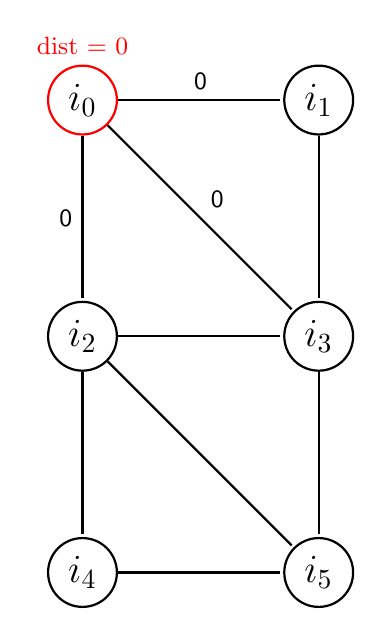
\begin{tikzpicture}[>=stealth',shorten >=1pt,auto,node distance=3cm,
            thick,main node/.style={circle,draw,font=\sffamily\Large\bfseries}]
            \node[main node, draw=red, label={[red]above:{\small dist = 0}}] (1) {$i_0$};
            \node[main node] (2) [right of=1] {$i_1$};
            \node[main node] (3) [below of=1] {$i_2$};
            \node[main node] (4) [below of=2] {$i_3$};
            \node[main node] (5) [below of=3] {$i_4$};
            \node[main node] (6) [below of=4] {$i_5$};
            \path[every node/.style={font=\sffamily\small}]
            (1) edge node [above] {0} (2)
            (1) edge node [left] {0} (3)
            (2) edge node [left] {} (4)
            (3) edge node [left] {} (4)
            (3) edge node [left] {} (6)
            (1) edge node [] {0} (4)
            (3) edge node [left] {} (5)
            (4) edge node [left] {} (6)
            (5) edge node [left] {} (6)
            ;
        \end{tikzpicture}
    \end{center}
\end{frame}

\begin{frame}{Breadth-First Search}{Simulation (2 of 6)}
    \begin{center}
        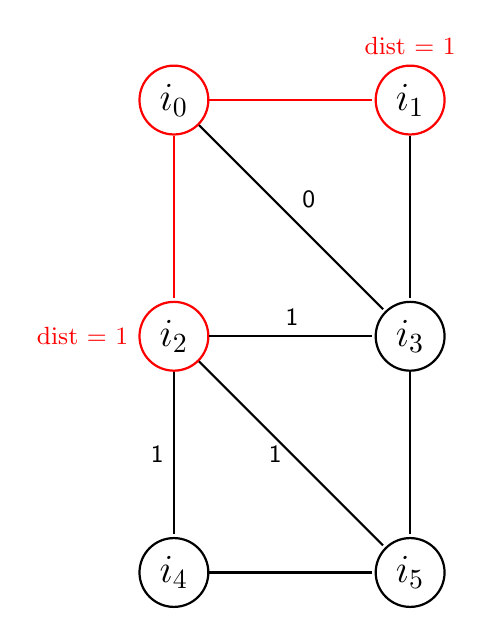
\begin{tikzpicture}[>=stealth',shorten >=1pt,auto,node distance=3cm,
        thick,main node/.style={circle,draw,font=\sffamily\Large\bfseries}]
        \node[main node, draw=red] (1) {$i_0$};
        \node[main node, draw=red, label={[red]above:{\small dist = 1}}] (2) [right of=1] {$i_1$};
        \node[main node, draw=red, label={[red]left:{\small dist = 1}}] (3) [below of=1] {$i_2$};
        \node[main node] (4) [below of=2] {$i_3$};
        \node[main node] (5) [below of=3] {$i_4$};
        \node[main node] (6) [below of=4] {$i_5$};
        \path[every node/.style={font=\sffamily\small}]
        (1) edge[red] node [left] {} (2)
        (1) edge[red] node [left] {} (3)
        (2) edge node [left] {} (4)
        (3) edge node [above] {1} (4)
        (3) edge node [left] {1} (6)
        (1) edge node [] {0} (4)
        (3) edge node [left] {1} (5)
        (4) edge node [left] {} (6)
        (5) edge node [left] {} (6)
        ;
        \end{tikzpicture}
    \end{center}
\end{frame}

\begin{frame}{Breadth-First Search}{Simulation (3 of 6)}
    \begin{center}
        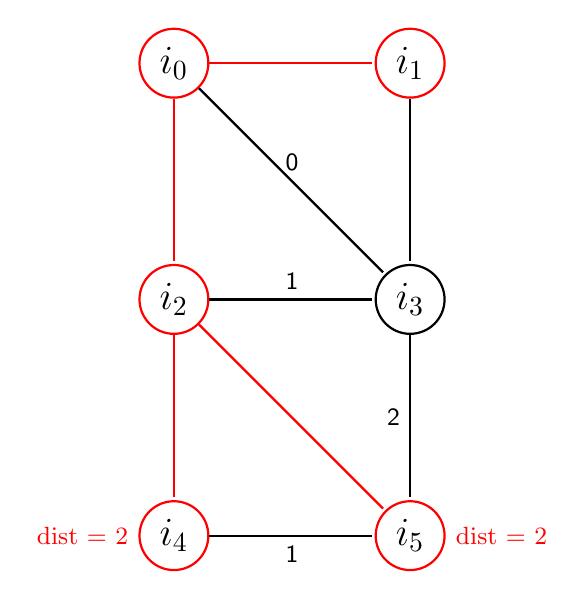
\begin{tikzpicture}[>=stealth',shorten >=1pt,auto,node distance=3cm,
        thick,main node/.style={circle,draw,font=\sffamily\Large\bfseries}]
        \node[main node, draw=red] (1) {$i_0$};
        \node[main node, draw=red] (2) [right of=1] {$i_1$};
        \node[main node, draw=red] (3) [below of=1] {$i_2$};
        \node[main node] (4) [below of=2] {$i_3$};
        \node[main node, draw=red, label={[red]left:{\small dist = 2}}] (5) [below of=3] {$i_4$};
        \node[main node, draw=red, label={[red]right:{\small dist = 2}}] (6) [below of=4] {$i_5$};
        \path[every node/.style={font=\sffamily\small}]
        (1) edge[red] node [left] {} (2)
        (1) edge[red] node [left] {} (3)
        (2) edge node [left] {} (4)
        (3) edge node [above] {1} (4)
        (3) edge[red] node [left] {} (6)
        (1) edge node [above] {0} (4)
        (3) edge[red] node [left] {} (5)
        (4) edge node [left] {2} (6)
        (5) edge node [below] {1} (6)
        ;
        \end{tikzpicture}
    \end{center}
\end{frame}

\begin{frame}{Breadth-First Search}{Simulation (4 of 6)}
    \begin{center}
        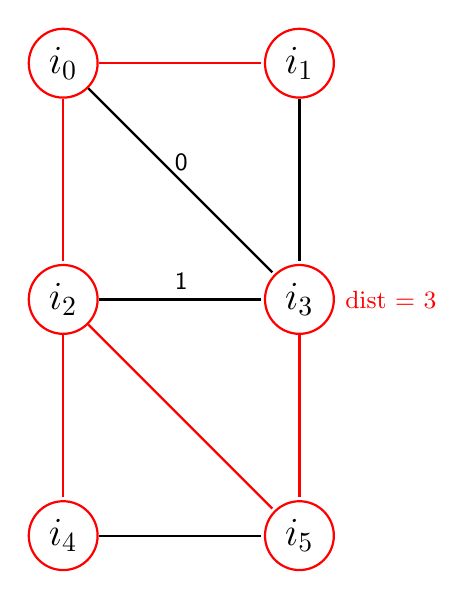
\begin{tikzpicture}[>=stealth',shorten >=1pt,auto,node distance=3cm,
        thick,main node/.style={circle,draw,font=\sffamily\Large\bfseries}]
        \node[main node, draw=red] (1) {$i_0$};
        \node[main node, draw=red] (2) [right of=1] {$i_1$};
        \node[main node, draw=red] (3) [below of=1] {$i_2$};
        \node[main node, draw=red, label={[red]right:{\small dist = 3}}] (4) [below of=2] {$i_3$};
        \node[main node, draw=red] (5) [below of=3] {$i_4$};
        \node[main node, draw=red] (6) [below of=4] {$i_5$};
        \path[every node/.style={font=\sffamily\small}]
        (1) edge[red] node [left] {} (2)
        (1) edge[red] node [left] {} (3)
        (2) edge node [left] {} (4)
        (3) edge node [above] {1} (4)
        (3) edge[red] node [left] {} (6)
        (1) edge node [above] {0} (4)
        (3) edge[red] node [left] {} (5)
        (4) edge[red] node [left] {} (6)
        (5) edge node [below] {} (6)
        ;
        \end{tikzpicture}
    \end{center}
\end{frame}

\begin{frame}{Breadth-First Search}{Simulation (5 of 6)}
    \begin{center}
        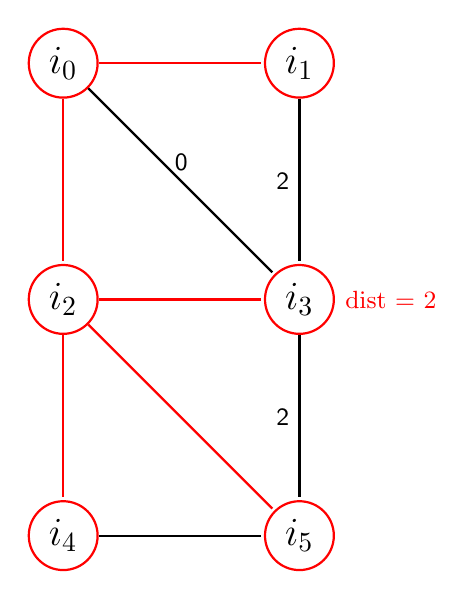
\begin{tikzpicture}[>=stealth',shorten >=1pt,auto,node distance=3cm,
        thick,main node/.style={circle,draw,font=\sffamily\Large\bfseries}]
        \node[main node, draw=red] (1) {$i_0$};
        \node[main node, draw=red] (2) [right of=1] {$i_1$};
        \node[main node, draw=red] (3) [below of=1] {$i_2$};
        \node[main node, draw=red, label={[red]right:{\small dist = 2}}] (4) [below of=2] {$i_3$};
        \node[main node, draw=red] (5) [below of=3] {$i_4$};
        \node[main node, draw=red] (6) [below of=4] {$i_5$};
        \path[every node/.style={font=\sffamily\small}]
        (1) edge[red] node [left] {} (2)
        (1) edge[red] node [left] {} (3)
        (2) edge node [left] {2} (4)
        (3) edge[red] node [above] {} (4)
        (3) edge[red] node [left] {} (6)
        (1) edge node [above] {0} (4)
        (3) edge[red] node [left] {} (5)
        (4) edge node [left] {2} (6)
        (5) edge node [below] {} (6)
        ;
        \end{tikzpicture}
    \end{center}
\end{frame}

\begin{frame}{Breadth-First Search}{Simulation (6 of 6)}
    \begin{center}
        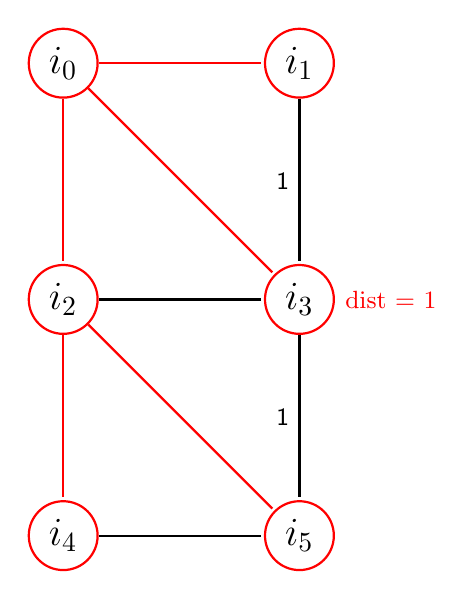
\begin{tikzpicture}[>=stealth',shorten >=1pt,auto,node distance=3cm,
        thick,main node/.style={circle,draw,font=\sffamily\Large\bfseries}]
        \node[main node, draw=red] (1) {$i_0$};
        \node[main node, draw=red] (2) [right of=1] {$i_1$};
        \node[main node, draw=red] (3) [below of=1] {$i_2$};
        \node[main node, draw=red, label={[red]right:{\small dist = 1}}] (4) [below of=2] {$i_3$};
        \node[main node, draw=red] (5) [below of=3] {$i_4$};
        \node[main node, draw=red] (6) [below of=4] {$i_5$};
        \path[every node/.style={font=\sffamily\small}]
        (1) edge[red] node [left] {} (2)
        (1) edge[red] node [left] {} (3)
        (2) edge node [left] {1} (4)
        (3) edge node [above] {} (4)
        (3) edge[red] node [left] {} (6)
        (1) edge[red] node [above] {} (4)
        (3) edge[red] node [left] {} (5)
        (4) edge node [left] {1} (6)
        (5) edge node [below] {} (6)
        ;
        \end{tikzpicture}
    \end{center}
\end{frame}

\begin{frame}{Breadth-First Search}{Results}
    \begin{columns}
        \column{.5\textwidth}
            Message Complexity: \\
            \hspace*{\parindent} $\mathbb{O}(n|E|)$ \\
            \pause
            \small
            Because each node can acquire different up to $n$ estimates of its distance to the starting node. In the worst case scenario, each estimate causes an update, each requiring at most $|E|$ messages to notify the adjacent nodes.
        \pause
        \column{.5\textwidth}
            \normalsize
            Time Complexity:
            \hspace*{\parindent} $\mathbb{O}(diam \times n(l + d))$ \\
            \pause
            \small
            Because the length of a shortest path from the starting node to any node is at most $diam$; and at most $n$ messages are ever in any channel. \\
           
    \end{columns} 
\end{frame}

\section{BellmanFord}
\begin{frame}{BellmanFord}{Algorithm}
    \normalsize
	The Bellman-Ford algorithm can be used to find a Minimum Spanning Tree. The network graph $G = (V, E)$ now also has weights $w_{i, j}$ for each edge $E_{i, j}$ going from vertex $i$ to $j$. The starting node $i_0$ is also required, once again. \\
    \vspace{12pt}
    \pause
	As in AsynchBFS, each process' code must account for erroneous assignments of the $parent$ variable, send out updates to its neighbors and wait for further corrections. \\
    \vspace{12pt}
    \pause
    A node therefore has no way to know when the algorithm has terminated. 
\end{frame}

\begin{frame}{BellmanFord}{Complexity}
	\textbf{Message Complexity}: \\
    \vspace{8pt}
    \pause
	$\mathbb{O}(n^n |E|)$ \\
    \vspace{8pt}
    \pause
    \small
    The number of messages sent on each channel $C_{i, j}$ is proportional to the number of different distance estimates the process $i$ receives. \\
    \vspace{8pt}
    \pause
    In the worst case, each estimate is better than the preceding one and it has to be propagated to all neighbors. \\
    \vspace{8pt}
    \pause 
    The number of different estimates received is bounded on the number of distinct single paths from $i_0$ to $i$ in the network graph: $\mathbb{O}(n^n)$.
\end{frame}

\begin{frame}{BellmanFord}{Complexity}
    \normalsize
    \textbf{Time Complexity}: \\
    \vspace{12pt}
    \pause
    $\mathbb{O}(n^{n+1}(l+d))$ \\
\end{frame}

\begin{frame}{Thank You!}
    \large
    Any questions?
\end{frame}

\end{document}
